\label{sec:eval}

We first analyze credential-management costs, then evaluate service invocation against NSC~\cite{meirovitch2021nsc}, an NDN remote code execution framework, and gRPC, an IP-based remote procedure call framework. The invocation experiments examine reliability under loss and provider unavailability, followed by the effects of ACK and provider-selection strategies.

\subsection{Credential Management Costs}
\label{sec:credential-cost}

For the same permission assignments, let $N$ be the number of entities, each holding at least one service permission, $p$ the average number of service permissions per entity, and $r$ the average number of roles per entity for which separate credentials are issued. A role may cover multiple services. We count credentials held by entities, not distinct shared service-key values across the deployment.

\begin{table}[t]
\centering
\caption{Entity-held credentials under shared identity trust}
\label{tab:credential-counts}
\small
\begin{tabularx}{\columnwidth}{@{}Xcc@{}}
\toprule
Credential category & NDNSF & Separate service keys \\
\midrule
Identity-signing credentials & $N$ & $N$ \\
Service-decryption credentials & $N$ & $Np$ \\
Subtotal & $2N$ & $N+Np$ \\
\bottomrule
\end{tabularx}
\end{table}

Table~\ref{tab:credential-counts} counts identity-signing and service-decryption credentials separately before adding them. Both configurations assume one active identity-signing credential per entity; a certificate and its associated private key are treated as one managed signing credential, not as one cryptographic key. NDNSF additionally assumes one ABE authority, one set of public parameters, and one current DKEY per entity. For 100 entities with 20 permissions each, the subtotals are 200 credentials for NDNSF and 2,100 for the separate-service-key configuration. These subtotals exclude content keys, additional encryption credentials, and authority-side material; any differences in those items must also be counted in a complete comparison.

Fewer credential objects do not necessarily mean fewer bytes or network messages. Let $L_i$ be the number of attribute occurrences in entity $i$'s access policy. For a construction whose key size grows linearly with $L_i$, total DKEY size is $\Theta(\sum_i L_i)$. If each policy lists its service permissions individually, this remains $\Theta(Np)$. DKEYs exceeding a Data packet's payload capacity require segmentation~\cite{dulal2023nac-abe}; separate-key deliveries can also be batched.

Granting another permission may require issuing a replacement DKEY containing the entity's updated policy. A separate-key design may instead deliver only the additional service key. Revocation that rotates the authority's parameters requires replacement DKEYs for every entity retaining permissions under that authority. Rotating only an affected service's shared key may require updates for fewer entities.

With a separately issued credential per assigned role, the role-credential count is $Nr$, or $\Theta(Nr)$. A role certificate may also be used to sign messages, so adding another $N$ identity credentials would double-count objects unless separate identity credentials are actually maintained. DNMP and trust schemas do not require a certificate per service~\cite{nichols2019dnmp,yu2015trust}; one role may cover several services. Role-based alternatives also need encryption for descriptor confidentiality, and those decryption credentials must be included when comparing complete configurations.

Aggregation reduces the number of decryption credentials to manage. Its overall cost depends on policy size, role reuse, and permission-change frequency.

\subsection{Trust-Rule Management Costs}
\label{sec:trust-rule-cost}

Trust-rule management must be counted separately from credential objects. DNMP compiles its VerSec schema into a signed binary representation for runtime use; its three-role prototype expresses the schema in 25 lines, excluding comments~\cite{nichols2019dnmp}. Parameterized rules can cover many identities, so neither DNMP nor NDNSF necessarily needs a separate trust rule for each entity or service permission.

Let $E$ denote the number of explicitly stored role--service authorization relationships. Listing these relationships requires $\Theta(E)$ entries, but does not imply $E$ independent schema rules: patterns or shared roles may express the same assignments more compactly. In NDNSF, individually listing each entity's service permissions requires $Np$ permission entries at the Controller, or $\Theta(Np)$, even though there are only $N$ DKEY objects. With fixed message formats and naming conventions, baseline signing rules in either design need not grow with $N$. NDNSF keeps service-permission lists in ABE policies; role-based designs can also change membership through credentials or authorization state without changing the schema. Changing a role's allowed actions may instead require a schema update.

For an update that delivers a complete $B$-byte signed schema to $V$ validators, the cumulative bytes received are $\Theta(VB)$. This is not the total network-link traffic, which depends on multicast, caching, and topology. A complete cost comparison must also include schema compilation, credential or DKEY updates, and permission-state distribution. Compilation and runtime validation costs must be measured separately; they cannot be inferred from credential or rule counts.

Keeping service-permission lists outside baseline signing rules does not eliminate permission-management costs; NDNSF manages them through ABE policies and keys. The invocation experiments do not measure key-distribution, schema-management, or revocation costs.


\subsection{Permission Aggregation: Measured Costs and Limits}
\label{sec:measured-permission-cost}

We compare eight identities with 1, 4 or 16 permissions under three C++ measurement configurations: one aggregated NAC-ABE DKEY per identity, separate NAC-ABE DKEYs per permission, and one RSA-protected bundle of AES service keys per identity. Five matched repetitions check authorized access, rejection of tampered data, rejection of new ciphertext by revoked holders retaining old keys, and surviving users' access after revocation.

At 16 permissions, initial local management CPU time, including key generation and recipient processing, is 303.10\,ms for aggregated ABE, 704.58\,ms for separate ABE keys and 6.15\,ms for batched RSA/AES. Aggregation lowers this cost relative to separate ABE keys, but the batched alternative has the lowest local cost in every measured phase.

A separate network comparison distributes pre-generated signed objects and excludes online generation. At 16 permissions, aggregation reduces initial management traffic from 281.72 to 86.74\,KiB relative to separate ABE keys (paired reduction 194.98\,KiB; 95\% interval 193.87--196.10), and revocation traffic from 247.11 to 75.80\,KiB. Eight aggregated DKEYs replace 128 separate DKEYs. At one permission, both ABE configurations use about 21.96\,KiB initially; a single new permission costs more under aggregation because it replaces a larger policy. The batched RSA/AES alternative uses only 27.25\,KiB initially and less traffic in every measured phase. Thus, aggregation helps relative to per-permission ABE when permissions are numerous, but is neither generally cheaper than batching nor free to update.

A separate MiniNDN~\cite{MININDN} experiment measures access recovery through the NDNSF Controller, Provider and User APIs, with five runs each at one and sixteen permissions per identity. All runs restore authorized access. At sixteen permissions, observed recovery takes 0.664--2.713\,s after a grant and 3.348--7.022\,s for the seven surviving users after revocation and key rotation. Calls using the pre-revocation permission state also complete after the revocation update, and some calls have no terminal result by the end of the observation window. These observations do not establish immediate revocation or uninterrupted service. This experiment does not compare management costs through the framework APIs across the three alternatives. Appendix~\ref{app:measured-permission-cost} gives the cost breakdown, reuse comparison and recovery details.

\subsection{Invocation Comparison Scope}

In the multi-provider comparisons with fixed-provider baselines, NSC and gRPC call one fixed provider, while NDNSF solicits several candidates and selects from their ACKs. NSC and NDNSF use signed NDN packets; NDNSF additionally uses NAC-ABE to protect service content. The matched multi-provider experiment below also enables failover in NSC and gRPC, but compares complete invocation paths rather than isolating feedback. These cross-framework comparisons do not isolate security overhead.
\subsection{Experimental Setup}

The original single-provider loss, fixed-provider, ACK-strategy, provider-selection, mobility and real-machine measurements used pre-provisioned certificates and excluded online certificate-chain retrieval and validation. They describe that implementation and do not quantify the current validation path. The no-loss single-provider and matched invocation studies use fixed-root certificate validation.

\begin{figure}[]
    \centering
    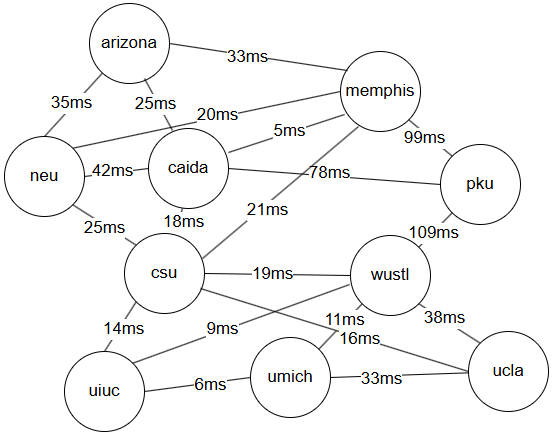
\includegraphics[width=0.4\textwidth]{figures/testbed_topo.png}
    \caption{Wired Network Topology}
    \label{fig:wired_topo}
    \vspace{-3mm}
\end{figure}

Figure~\ref{fig:wired_topo} illustrates the emulated wired network used in the wired invocation experiments unless otherwise specified, derived from a subset of the global NDN Testbed topology~\cite{testbedtopo}. All nodes are connected by 1~Gbps wired links, with per-link latency configured according to the values shown in the topology. Unless otherwise specified, all links are lossless; in lossy wired network experiments, a uniform packet loss rate of 1\% is applied to every link.

\begin{figure}[]
    \centering
    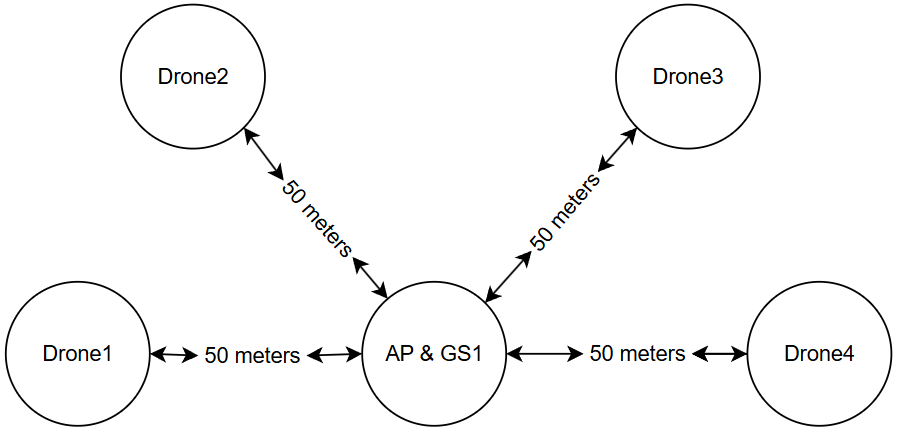
\includegraphics[width=0.4\textwidth]{figures/WIFI_TOPO.png}
    \caption{Wireless Network Topology}
    \label{fig:wifi_topo}
    \vspace{-3mm}
\end{figure}

Figure~\ref{fig:wifi_topo} depicts the emulated wireless network. All drones initially start 50~meters from the ground station and then move randomly within a 400\,m $\times$ 400\,m area centered at the ground station following the Random Waypoint mobility model. The WiFi access point (AP) is colocated with the ground station, and its communication range is varied across experiments. Drones moving outside the AP range cannot receive packets, resulting in mobility-induced packet loss.

In addition to the emulation experiments, we conduct real-world experiments using a Lenovo Y70 laptop, a desktop PC equipped with an AMD Ryzen 7 3700X processor, and an Odroid C4 device. The PC is connected directly to a WiFi AP over Ethernet, whereas the laptop and Odroid C4 communicate wirelessly through the same AP.

In the single-provider, fixed-provider, ACK-strategy, provider-selection, mobility and real-machine comparisons, NDNSF users employ the first-responding provider-selection strategy unless otherwise specified. By default, providers acknowledge and serve all incoming requests. Each service request incurs a 5\,ms processing delay at the provider to emulate service execution overhead. Except for the no-loss single-provider comparison, these experiments use a 512~B publication-embedding threshold, which limits the encoded Data size eligible for carriage in Sync Interests. The targeted, matched-availability, advertisement and permission studies specify their own workloads and completion criteria.
\subsection{Performance Metrics}

We use the following metrics in our evaluation:

\begin{enumerate}
\item \textbf{Service Latency}: the time interval from initiating a service request to receiving the service result.

\item \textbf{Success Rate}: the proportion of measured service requests for which the user accepts a result under the invocation's configured timeout handling. A request counts once, regardless of message retrieval retries. A timeout does not establish whether the provider executed the request.
\end{enumerate}

The single-provider, fixed-provider, ACK-strategy, provider-selection, mobility and real-machine comparisons report point estimates without repetition-based uncertainty estimates. They do not establish statistical differences or isolate authorization costs. The matched studies report repetitions and uncertainty.

\subsection{Wired Evaluation Results with One Provider}

\begin{figure}[!h]
  \centering
  \begin{tikzpicture}
    \begin{axis}[
      ybar,
      ymin=0,
      ymax=280,
      xlabel={Requests Per Second},
      ylabel={Service Latency (ms)},
      symbolic x coords={10,30,50,70},
      xtick=data,
      ytick={0,50,100,150,200,250},
      label style={font=\footnotesize},
      tick label style={font=\footnotesize},
      nodes near coords,
      nodes near coords style={font=\tiny,
        /pgf/number format/fixed, /pgf/number format/precision=0},
      nodes near coords align={vertical},
      legend style={
        at={(0.5,1.03)},
        anchor=south,
        legend columns=2,
        draw=none,
        font=\footnotesize,
        /tikz/every even column/.append style={column sep=6pt}
      },
      bar width=7pt,
      height=0.70\columnwidth,
      width=\columnwidth,
      enlarge x limits={0.18},
      ]
      \addplot[pattern=north east lines,pattern color=black]
        coordinates {(10,217.840) (30,210.937) (50,212.190) (70,215.500)};
      \addplot[fill=gray]
        coordinates {(10,116.204) (30,107.600) (50,111.480) (70,113.300)};
      \addplot[fill=white]
        coordinates {(10,226.449) (30,223.768) (50,218.264) (70,237.604)};
      \addplot[pattern=dots,pattern color=black]
        coordinates {(10,119.092) (30,115.440) (50,117.359) (70,117.489)};
      \legend{NSC,gRPC,NDNSF,NDNSF-Targeted}
    \end{axis}
  \end{tikzpicture}
  \caption{Average Service Latency in Wired Network (Link Loss=0\%); this experimental data was collected between two nodes: Memphis and UCLA.}
  \label{fig:latency_0.00}
  \vspace{-3mm}
\end{figure}

In the no-loss comparison, Memphis and UCLA act as the service user and provider, respectively. NDNSF, NDNSF-Targeted, NSC and gRPC use the same rates of 10, 30, 50 and 70 requests per second (RPS), with a 64~B echo workload and 5\,ms service delay. A timer submits requests without waiting for earlier calls to finish. Each measurement lasts 60\,s after a 10\,s warmup; the request deadline is 5\,s. NDNSF users and providers use ECDSA runtime signatures and separate RSA keys for NAC-ABE credential delivery, with fixed-root certificate validation and a 4096~B publication-embedding threshold. NSC validates signed packets against pinned ECDSA keys, and gRPC uses mutual TLS.

Figure~\ref{fig:latency_0.00} shows that NDNSF's four-step invocation has roughly twice the mean latency of two-step targeted invocation at 10--70 RPS: 218--238\,ms versus 115--119\,ms. During measurement, all targeted calls use the Request--Response path. NDNSF has higher mean latency than NSC, while gRPC has the lowest mean latency at each rate. All four configurations submit every scheduled request and complete all measured calls within the 5\,s deadline.

\begin{figure}[!h]
  \centering
  \begin{tikzpicture}
    \begin{axis}[
      ybar,
      ymin=0,
      ymax=125, % Shifted up slightly to guarantee breathing room for staggered 100s
      xlabel={Requests Per Second},
      ylabel={Success Rate (\%)},
      symbolic x coords={10,30,50,70},
      xtick=data,
      label style={font=\footnotesize},
      tick label style={font=\footnotesize},
      nodes near coords,
      % Stagger the labels so the duplicate 100 values don't collide horizontally
      nodes near coords style={
        font=\tiny,
        every node near coord/.append style={
          yshift={
            \ifnum\plotnum=1 6pt\else\ifnum\plotnum=2 1pt\else 1pt\fi\fi
          }
        }
      },
      nodes near coords align={vertical},
      legend style={
        at={(0.5,1.05)}, 
        anchor=south,
        legend columns=-1,
        draw=none,
        font=\footnotesize,
        /tikz/every even column/.append style={column sep=5pt}
      },
      bar width=9pt, % Tightened to perfectly match your 0.40\textwidth scale
      height=0.30\textwidth, 
      width=0.40\textwidth,
      enlarge x limits={0.25}, 
      ]
      \addplot[pattern=north east lines,pattern color=black] coordinates {(10,87) (30,87) (50,87) (70,88)};
      \addplot[fill=gray] coordinates {(10,100) (30,100) (50,100) (70,100)};
      \addplot[fill=white] coordinates {(10,100) (30,100) (50,100) (70,100)};
      \legend{NSC,gRPC,NDNSF}
    \end{axis}
  \end{tikzpicture}
  \caption{Success Rate in Wired Network (Link Loss=1\%, earlier implementation); this experimental data was collected between two nodes: Memphis and UCLA.}
  \label{fig:success_rate_0.01}
  %\vspace{-3mm}
\end{figure}

The separate 1\% link-loss comparison uses the earlier implementation with the 512~B publication-embedding threshold and pre-provisioned certificate configuration described above. Figure~\ref{fig:success_rate_0.01} shows that both gRPC and NDNSF maintain a 100\% success rate across all request rates. In contrast, NSC experiences 12--13\% request failures under the tested retry and timeout configuration. NDNSF therefore matches TCP-based gRPC's completion rate in that configuration.

\subsection{Reliability Under Intermittent Provider Failures}
\label{sec:intermittent-provider-failures}

\begin{table}[t]
  \centering
  \caption{
    Service Request Success Rate (\%) under Intermittent Provider Failures in a Wired Multi-Provider Environment
    %Each provider independently enters a temporary unavailable state with the specified probability.
  }
  \label{tab:success_rate_wired_intermittent}

  \small
  \setlength{\tabcolsep}{8pt}

  \begin{tabular}{lccc}
    \toprule

    \multirow{2}{*}{System}
      & \multicolumn{3}{c}{Provider Failure Probability} \\

    \cmidrule(lr){2-4}

      & 10\%
      & 20\%
      & 30\% \\

    \midrule

    NSC
      & 83.25
      & 66.58
      & 49.92 \\

    gRPC
      & 83.35
      & 66.69
      & 65.36 \\

    \textbf{NDNSF}
      & \textbf{99.82}
      & \textbf{99.46}
      & \textbf{96.70} \\

    \bottomrule
  \end{tabular}
  \vspace{-3mm}
\end{table}

In this experiment, UCLA, WUSTL, and UIUC provide identical services to Memphis. Both gRPC and NSC bind Memphis to the UCLA provider, whereas NDNSF uses the first-responding strategy to dynamically select among multiple providers. To emulate intermittent service availability, each provider independently enters a 10-second rejection period when it is unable to serve incoming requests with probability 10\%, 20\%, or 30\% every 10 seconds. For NDNSF, unavailable providers suppress ACKs, allowing the user to select another available provider when possible.

Table~\ref{tab:success_rate_wired_intermittent} shows that NDNSF achieves higher completion rates than the fixed-provider NSC and gRPC configurations at all tested rejection probabilities. When the rejection probability is 20\%, NDNSF maintains a 99.46\% success rate, while NSC and gRPC achieve only 66.58\% and 66.69\%, respectively. Even at a 30\% rejection probability, NDNSF still achieves 96.70\% success. This improvement comes from NDNSF's one-to-many service invocation model: a request can use another available provider if selection and execution finish before timeout. In contrast, the configured gRPC and NSC clients are bound to a single provider, so requests fail whenever that provider is unavailable.

\subsection{Task-Feedback Ablation}
\label{sec:task-feedback-ablation}

To isolate task feedback from access to alternative providers, we used an internal NDNSF ablation in five paired MiniNDN blocks of 13 planned tasks each. Both arms used the same two candidates, protected Request--ACK--Selection--Response path, fixed-root validation, task-state trace, 64-byte input, simulated 5-ms handler, and modeled 2-s target-recognition deadline. In both arms, the user selected the lowest provider name among the collected valid positive ACKs. Only the Provider's participation decision differed: a current-task capacity check versus ACK-all.

Each 60\,s block schedules tasks every 4.7\,s, with at most three invocation attempts per task; an attempt is a new invocation, not a message-retrieval retry. Three 1\,Gbps links have 10\,ms one-way delay and no random loss. Both providers remain reachable. Their complementary capacity states alternate at intervals of 0.3--0.7\,s (mean 0.5\,s), with each provider constrained half the time. A constrained provider cannot accept its compute- or memory-specialty task, while the other remains eligible.

Task feedback produced 65/65 timely correct completions versus 57/65 for ACK-all (paired gain 12.3 percentage points; block-bootstrap 95\% interval 7.7--18.5). It required 65 versus 89 attempts; 32 ACK-all attempts were rejected for insufficient capacity, versus none with feedback. Neither arm had duplicate or late eligible execution. Mean per-attempt submission-to-Selection time was 83.9 versus 50.1\,ms; gross relay IP traffic was 71.9 versus 99.2\,KiB per planned task. Feedback improved completion and reduced failed attempts in these traces at about 34\,ms additional selection delay. The result does not establish the same gain for other loads or deadlines.

\subsection{Matched Multi-Provider Availability}
\label{sec:matched-provider-availability}

We next compare the full NDNSF invocation path with NSC and gRPC clients that can switch between the same two providers. The testbed uses three 1\,Gbps links with 10\,ms one-way delay and no random packet loss; the offline conditions additionally apply the scheduled disconnections. Five paired MiniNDN runs per condition use the same scheduled arrivals, provider-state trace, 64-byte input, simulated 5\,ms handler and 2\,s deadline from scheduled arrival. Each 60\,s run schedules 13 tasks at 4.7\,s intervals. The conditions are stable availability, slow or fast link disconnection, and fast online busy rejection. In the offline conditions, complementary link states leave exactly one provider reachable, with each reachable half the time. State intervals average 5\,s (slow) or 0.5\,s (fast); online busy rejection uses the fast trace to alternate which provider rejects all tasks.

NDNSF uses Request--ACK--Selection--Response; NSC and gRPC retry with another provider after a failed attempt. NDNSF permits at most three invocation attempts per task; NSC and gRPC try each provider at most once (two attempts). After a timeout with possible execution, the NDNSF client keeps the attempt open until the task deadline; it retries only when non-execution is established. NDNSF allows 250\,ms for ACK collection and sets an initial 600\,ms attempt timeout, while NSC and gRPC use 250\,ms per attempt. Their security mechanisms also differ, so this comparison does not isolate cryptographic overhead. Here, correct completion requires a timely validated result without late or duplicate eligible handler execution; all planned tasks remain in the denominator. Table~\ref{tab:matched-provider-availability} reports the results.

\begin{table}[!ht]
  \centering
  \caption{Matched multi-provider results (65 tasks per arm and condition). Latency includes a 2\,s penalty for failures; gross relay IP includes background traffic.}
  \label{tab:matched-provider-availability}
  \footnotesize
  \setlength{\tabcolsep}{2.5pt}
  \begin{tabular}{lccc}
    \toprule
    \multicolumn{4}{l}{Correct tasks/65 (mean latency, ms)} \\
    Condition & NDNSF & NSC & gRPC \\
    \midrule
    Stable & 65/65 (121.6) & 65/65 (104.6) & 65/65 (56.4) \\
    Slow offline & 63/65 (374.3) & 64/65 (255.3) & 55/65 (364.6) \\
    Fast offline & 35/65 (1124.3) & 43/65 (798.5) & 31/65 (1122.2) \\
    Fast busy & 65/65 (249.5) & 63/65 (197.7) & 65/65 (82.4) \\
    \midrule
    \multicolumn{4}{l}{Gross relay IP (KiB/task)} \\
    Condition & NDNSF & NSC & gRPC \\
    \midrule
    Stable & 73.0 & 6.4 & 41.3 \\
    Slow offline & 50.9 & 6.7 & 32.2 \\
    Fast offline & 49.8 & 5.3 & 30.1 \\
    Fast busy & 88.2 & 7.6 & 39.7 \\
    \bottomrule
  \end{tabular}
\end{table}

We assess completion from task plans, handler records and terminal states, and measure traffic from packet captures. Under slow disconnection, NDNSF completes 63/65 tasks, versus 64/65 for NSC and 55/65 for gRPC (NDNSF--gRPC paired difference 12.3 percentage points; block-bootstrap 95\% interval 7.7--18.5). Under fast disconnection, NDNSF completes 35/65 versus 43/65 and 31/65; its paired difference from NSC is $-12.3$ points (interval $-26.2$ to 1.5), without an established completion advantage. NDNSF has no observed duplicate or late eligible execution. NSC and gRPC each have one duplicate execution under slow disconnection; gRPC has three under fast disconnection. In stable conditions, all three complete 65/65; under online busy rejection, their counts are 65/65, 63/65 and 65/65. NDNSF has higher mean latency and gross relay traffic in all four conditions. Different retry policies, per-attempt timeouts and transport paths prevent attributing these cross-system results to feedback alone.

We also compare five paired blocks with both providers reachable and task-specific capacity varying on the same fast trace: a constrained provider cannot accept its compute- or memory-specialty task, while the other provider remains eligible. Task classes follow a seed-shifted compute--compute--memory--memory cycle, while the NSC and gRPC clients rotate their default provider order across tasks. Generic gRPC health checks report reachability; NSC discovers task rejection after input delivery, while NDNSF receives it in ACK feedback. With the same 2\,s deadline, all three arms correctly complete 65/65 tasks without duplicate or late execution. NDNSF makes 71 attempts, versus 80 for NSC and 78 for gRPC, but its mean latency is 218.0\,ms versus 180.4 and 94.7\,ms, and gross relay IP is 78.6 versus 7.8 and 40.9\,KiB per planned task. All tasks finish within 521\,ms under this 64-byte, 5-ms-handler workload, leaving ample deadline slack. Thus, feedback avoids some retries here without improving deadline completion or offsetting its coordination cost.

\subsection{Solicitation Versus Coarse Service Advertisements}
\label{sec:dynamic-selection-cost}

We compare task-specific solicitation with preselection from long-term service advertisements followed by protected targeted requests. The advertisement arm queries status after a failed call; its change-driven publications model service capabilities, not an unmodified NDNSD implementation. In five paired blocks, two providers receive one synthetic task per second with a 2\,s deadline and an 80\,ms simulated handler. Both arms use the same eligibility checks and at most three attempts. The solicitation client waits until the task deadline if an unanswered attempt may have executed; the advertisement client can retry a targeted call after its attempt timeout. These are simulated resource and link conditions, not measured inference or flight workloads.

When temporary busy periods change task eligibility, both arms correctly complete 300/300 tasks; solicitation uses fewer submissions (313 versus 408) but more relay traffic (74.2 versus 56.5\,KiB per task). Mean latencies are 272.2 and 247.7\,ms, with no resolved paired latency difference. When complementary provider links alternate between reachable and unreachable, leaving one reachable at a time, solicitation completes 259/300 versus 270/300 tasks within 2\,s (paired difference $-3.7$ percentage points; 95\% interval $-5.3$ to $-1.7$). Its mean latency including the 2\,s failure penalty is lower (642.6 versus 732.3\,ms), but it uses more relay traffic (50.1 versus 42.1\,KiB per task). Solicitation has no observed duplicate or late eligible execution; one duplicate execution with advertisements is excluded from correct completion. Solicitation completes fewer tasks under these link changes. The comparison also changes invocation paths, retry behavior and advertisement visibility, so it does not isolate feedback alone.

\subsection{Reliability Under Mobility-Induced Disconnections}
\label{sec:mobility-induced-disconnections}

In the wireless experiments, the ground station acts as the user and the drones act as providers. The AP WiFi range is varied from 100\,m to 200\,m in the simulated coverage model. When a drone moves outside the coverage area, it becomes temporarily unavailable.

\begin{table}[!ht]
  \centering
  \caption{
    Service Request Success Rate (\%) in a Wireless Mobile Network with Different WiFi Ranges
  }
  \label{tab:success_rate_wifi_mobile}

  \small
  \setlength{\tabcolsep}{9pt}

  \begin{tabular}{lccc}
    \toprule

    \multirow{2}{*}{System}
      & \multicolumn{3}{c}{AP WiFi Range} \\

    \cmidrule(lr){2-4}

      & 100\,m
      & 150\,m
      & 200\,m \\

    \midrule

    NSC
      & 45.42
      & 68.75
      & 88.33 \\

    gRPC
      & 45.23
      & 68.05
      & 87.14 \\

    \textbf{NDNSF}
      & \textbf{96.25}
      & \textbf{100.00}
      & \textbf{100.00} \\

    \bottomrule
  \end{tabular}
\end{table}

Table~\ref{tab:success_rate_wifi_mobile} shows that NDNSF achieves higher success rates than the fixed-provider NSC and gRPC configurations under the tested mobility-induced disconnections. With a 100\,m WiFi range, NDNSF achieves a 96.25\% success rate, compared to 45.42\% for NSC and 45.23\% for gRPC. As the WiFi range increases, the success rates of all systems improve, with NDNSF having the highest reported rates in these configurations, reaching 100\% at both 150\,m and 200\,m.

This advantage stems from NDNSF's one-to-many service model. The ground station can dynamically select among multiple drones, allowing requests to use another reachable drone before timeout. In contrast, the configured gRPC and NSC clients bind the ground station to a single drone, making them more vulnerable to mobility-induced disconnections.


\subsection{ACK Strategy Evaluation}
\label{sec:selective-ack}

This experiment evaluates NDNSF's Selective ACK mechanism in a multi-provider environment. Memphis acts as the service user with a request rate of 50~RPS, while CSU, UCLA, and WUSTL provide identical services. CSU is the closest provider but is intentionally overloaded: although it continues receiving requests, it delays responses by 30~seconds. Since the request timeout is 5~seconds, requests handled by CSU are expected to fail.  We compare two ACK mechanisms. Under \emph{ACK-all}, every provider always returns an ACK, even when they cannot complete requests before timeout. Under \emph{Selective ACK}, providers suppress ACKs when overloaded, preventing themselves from being selected.

Table~\ref{tab:selective-ack} shows that ACK-all performs poorly because the first-responding strategy selects CSU for 2209 out of 2250 requests, all of which fail to return a response before the timeout, resulting in only a 1.82\% success rate. In contrast, Selective ACK prevents CSU from being selected while overloaded, allowing requests to be handled by UCLA and WUSTL and achieving a 100\% success rate. Under this forced-overload configuration, suppressing CSU's ACK prevents the first-responding strategy from choosing it.

\begin{table}[]
  \centering
  \caption{Impact of ACK Strategy When the Nearest Provider is Overloaded}
  \label{tab:selective-ack}
  \setlength{\tabcolsep}{4pt}

  \begin{tabular}{l r r r}
    \toprule
    Mechanism &
    Success &
    Selection Distribution \\
    &
    Rate &
    CSU/UCLA/WUSTL \\
    \midrule
    ACK-all       & 1.82\% & 2209/34/7 \\
    Selective ACK  & 100.00\% & 0/1723/527 \\
    \bottomrule
  \end{tabular}
  \vspace{-3mm}
\end{table}

\subsection{Provider-Selection Strategy Evaluation}
\label{sec:custom-selection}

This experiment evaluates NDNSF's customizable provider-selection mechanism. Memphis acts as the service user, while UIUC, UCLA, and WUSTL provide the same service. To create heterogeneous provider conditions, UIUC, the closest provider, is configured with the slowest service-processing delay (100\,ms), while UCLA and WUSTL use delays of 20\,ms and 5\,ms, respectively. Each provider returns ACKs carrying metadata containing current queue size. We compare two provider-selection strategies. \emph{First-Responding} selects the first provider returning a valid ACK, minimizing ACK waiting time but favoring nearby providers even when they have slower service execution. In contrast, \emph{Shortest-Queue-First}  selects the provider with the smallest reported queue.

\begin{figure}[!hb]
  \centering
  \begin{tikzpicture}
    \begin{axis}[
      ybar,
      ymin=0,
      ymax=360,
      xlabel={Requests Per Second},
      ylabel={Average Latency (ms)},
      symbolic x coords={10,30,50},
      xtick=data,
      nodes near coords,
      nodes near coords align={vertical},
      every node near coord/.append style={font=\tiny},
      legend style={at={(0.5,1.05)},
        anchor=south,legend columns=-1,draw=none},
      bar width=12pt,
      height=0.30\textwidth,
      width=0.40\textwidth,
      enlarge x limits={0.25},
      ]
      \addplot[pattern=north east lines,pattern color=black]
        coordinates {(10,275.65) (30,282.96) (50,317.50)};
      \addplot[fill=gray]
        coordinates {(10,223.65) (30,233.42) (50,299.76)};
      \legend{First-Responding, Shortest-Queue-First}
    \end{axis}
  \end{tikzpicture}
  \caption{Average Service Latency under First-Responding and Shortest-Queue-First Provider-Selection Strategies}
  \label{fig:custom-selection-avg-latency}
\end{figure}

Figure~\ref{fig:custom-selection-avg-latency} shows lower mean latency with Shortest-Queue-First at each tested rate; at 10~RPS, it is 223.65\,ms versus 275.65\,ms with First-Responding. In this configuration, using queue information offsets the additional ACK-collection delay.

\subsection{Real-World Experiments}

In the real-world experiments, the Odroid C4 acts as the service user, while the laptop and PC act as service providers. To evaluate robustness under intermittent service availability, the laptop is unavailable during the first half of the experiment, while the PC is unavailable during the middle half, leaving both providers simultaneously available only during the last quarter of the run. For gRPC and NSC, the Odroid C4 is bound to the laptop provider. In contrast, NDNSF allows both the laptop and PC to provide service to the Odroid C4.

\begin{table}[!ht]
  \centering
  \caption{Service Availability in Real-World Experiments}
  \label{tab:real_machine_availability}

  \small
  \setlength{\tabcolsep}{9pt}

  \begin{tabular}{lcc}
    \toprule
    System & 10 RPS & 30 RPS \\
    \midrule
    NSC   & 52.67\% & 51.78\% \\
    gRPC  & 49.33\% & 47.06\% \\
    \textbf{NDNSF} & \textbf{74.62\%} & \textbf{73.73\%} \\
    \bottomrule
  \end{tabular}
  \vspace{-3mm}
\end{table}

Table~\ref{tab:real_machine_availability} reports the resulting service request success rates. Because gRPC and NSC rely on a fixed provider, their success rates remain near 50\%, matching the provider availability period. NDNSF can select a reachable provider when one is available, achieving a success rate close to the expected 75\% service-availability window. This comparison supports the benefit of access to alternative providers, but does not isolate task-specific feedback.
